\RequirePackage[l2tabu,orthodox]{nag}
\documentclass{IEEEtran}
\usepackage{fullpage}
\usepackage{graphicx}
\usepackage{hyperref}
\usepackage{listings}
\usepackage{mathtools}
\usepackage{microtype}
\usepackage{pgfplots}
\usepackage{tikz}

\pgfplotsset{compat=newest}
\usetikzlibrary{positioning}

\title{Fashion MNIST: A Class Project}
\author{Andrew Cousino}

\bibliographystyle{ieeetr}

\def\layersep{1.4cm}
\newcommand{\lt}{\symbol{"3C}}
\newcommand{\gt}{\symbol{"3E}}
\DeclareMathOperator{\rot}{rot}

\begin{document}
\lstset{language=Python,frame=lines}
\maketitle

\begin{abstract}
In this work, we construct a simple neural network to classify images from the
Fashion MNIST data set \cite{xiao2017fashionmnist}. This work was done for
personal interest and as a project for the EECS 740 course at the University
of Kansas.
\end{abstract}

\section{Introduction}
For personal interest and as a project for EECS 740 at the University of Kansas,
the author has constructed a simple neural network to classify images in the
Fashion-MNIST data set. Fashion-MNIST \cite{xiao2017fashionmnist} is a
collection of \(70,000\) \(28\times 28\) grayscale images each representing a
fashion product from 10 different categories. The set is split into a \(60,000\)
image training set and a \(10,000\) image testing set. Each image is normalized
as described in \cite{xiao2017fashionmnist}. The categories are as listed in
table \ref{table:categories} with sample images shown in figure
\ref{fig:sample}. Fashion-MNIST is intended to be a drop in replacement for the
MNIST handwriting recognition data set, a similar data set of images of
handwritten digits. The MNIST data set is seen as too easy with simple
convolutional neural networks achieving 99.7\% accuracy.

\begin{table}[h]
    \centering
    \begin{tabular}{rl}
        0 & Top or T-shirt \\
        1 & Trouser \\
        2 & Pullover \\
        3 & Dress \\
        4 & Coat \\
        5 & Sandal \\
        6 & Shirt \\
        7 & Sneaker \\
        8 & Bag \\
        9 & Ankle boot \\
    \end{tabular}
    \caption{Fashion MNIST Categories}
    \label{table:categories}
\end{table}

\begin{figure}
    \centering
    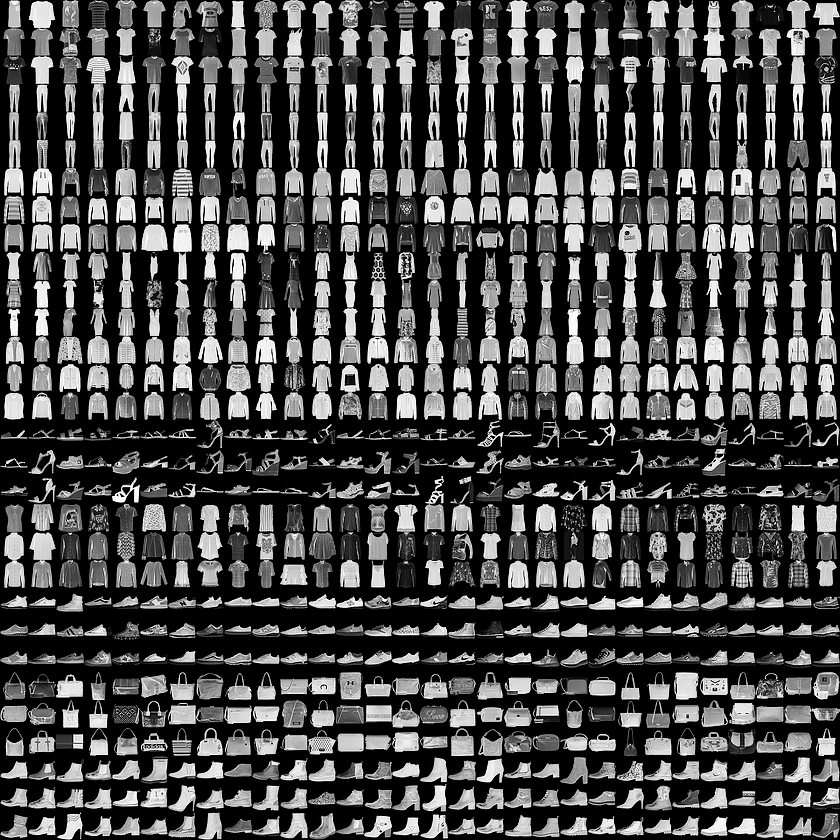
\includegraphics[width=0.45\textwidth]{fashion-mnist-sprite.png}
    \caption{Sample of Fashion MNIST images with each class taking 3 rows}
    \label{fig:sample}
\end{figure}

Other important image recognition data sets mentioned in the Related Works
section are CIFAR-10, CIFAR-100, ImageNet, and SVHN. The CIFAR data sets are
for image classification with classes numbering 10 and 100 respectively.
ImageNet is another image classification data set contains more than \(20,000\)
classes. And SVHN is the Google Street View image recognition data set of house
numbers where the task is to detect and classify house numbers from each image.

Neural networks have proven to be very useful for image classification as seen
in \cite{Zagoruyko_2016}, \cite{xie2019selftraining},
\cite{byerly2020branching}, \cite{sabour2017dynamic}, and
\cite{zhong2017random}. The architecture for neural networks is inspired by how
information is processed in the brain, using many layers to learn features at
increasing levels of abstractions. The base elements of neural networks are
artifical neurons, also called perceptrons. The connection between perceptrons
are called weights. The inputs to a perceptron are linearly combined with the
weights, sometimes offset by a bias, and sent through a pre-determined
non-linear function called an activation function. The network learns the values
of the weights and biases through a training process called backpropogation.
Backpropogation typically uses gradient descent trying to minimize a fixed loss
function.

\section{Background}
\subsection{Artificial Neural Networks}
The artificial neural network in figure \ref{fig:neural_network} is a simple
network with a single hidden layer. In general, we have \(L\) layers with layer
\(1\) being the input layer and \(L\) being the output layer. Let
\(w_{ij}^{l}\) be the weight between the \(i\)th node, or perceptron, in the
\(l - 1\)th layer and the \(j\)th perceptron in the \(l\)th layer, and let
\(b_{i}^{l}\) be the bias associated with the \(i\)th perceptron in the \(l\)th
layer. The activation \(a_{i}^{l}\) of the \(i\)th perceptron in the \((l+1)\)st
layer is recursively defined as
\[a_{i}^{l + 1}\coloneqq \sigma\left(\sum_{j} w_{i j}^{l + 1} a_{j}^{l}
 + b_{i}^{l + 1}\right)\text{,}\]
where \(\sigma\) is the activation function. The chosen activation function is
always a non-linear, differentiable function. Historically, it has been the
sigmoid function \(z\mapsto 1/(1 + e^{-z})\). Recently, the rectified linear
unit, or ReLU, \(z\mapsto \max\{0, z\}\) has been the preferred choice. If we
vectorize the activation function so that \(\sigma(z)\) is the function
\(\sigma\) applied to the vector \(z\) element-by-element, then we can rewrite
the activation equation as 
\begin{equation}
    a^{l+1}\coloneqq \sigma \left(w^{l + 1} a^{l} + b^{l + 1}\right)\text{.}
    \label{eqn:forward}
\end{equation}
By letting \(z^{l + 1}\coloneqq w^{l + 1} a^{l} + b^{l + 1}\), this can be
further simplified to \(a^{l + 1} = \sigma z^{l + 1}\).

\begin{figure}
    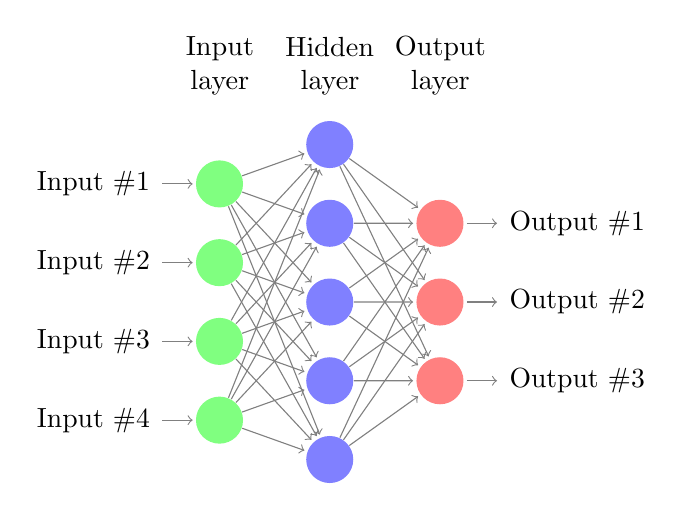
\begin{tikzpicture}[shorten >= 1pt, ->, draw=black!50, node distance=\layersep]
        \tikzstyle{every pin edge}=[<-,shorten <= 1pt];
        \tikzstyle{neuron}=[circle,fill=black!50,minimum size=17pt,inner sep=0pt];
        \tikzstyle{input neuron}=[neuron, fill=green!50];
        \tikzstyle{output neuron}=[neuron, fill=red!50];
        \tikzstyle{hidden neuron}=[neuron, fill=blue!50];
        \tikzstyle{annot}=[text width=4em, text centered];

        % input layer neurons
        \foreach \name / \y in {1,...,4}
            \node[input neuron,pin=left:Input \#\y] (I-\name) at (0, -0.5-\y) {};
        % hidden layer neurons
        \foreach \name / \y in {1,...,5}
            \node[hidden neuron] (H-\name) at (\layersep, -\y cm) {};
        % output layer neurons
        \foreach \name / \y in {1,2,3}
            \node[output neuron,pin={[pin edge={->}]right:Output \#\y}] (O-\name) at (2*\layersep, -1-\y) {};
        % Connect input layer and hidden layer
        \foreach \source in {1,...,4}
            \foreach \dest in {1,...,5}
                \path (I-\source) edge (H-\dest);
        % Connect hidden layer to output layer
        \foreach \source in {1,...,5}
            \foreach \dest in {1,...,3}
                \path (H-\source) edge (O-\dest);
        % Annotate layers
        \node[annot,above of=H-1, node distance=1cm] (hl) {Hidden layer};
        \node[annot,left of=hl] {Input layer};
        \node[annot,right of=hl] {Output layer};
    \end{tikzpicture}
    \caption{A neural network with one hidden layer}
    \label{fig:neural_network}
\end{figure}

Let \(y(x)\) be the output for the training input \(x\), and \(a^{L}(x)\) be the
output of the neural network. We define the loss, or error, of the neural
network to be
\[\mathcal{L}\coloneqq \frac{1}{2}\sum_{x}{\left\| y(x)
 - a^{L}(x)\right\|}^{2}\text{.}\]
This is known as the \(\ell_{2}\) loss function. There are many loss functions
to choose, the main requirement is that it be partially differentiable with
respect to the activations. This is so that backpropogation can occur to
update the weights and biases.

Backpropogation occurs by first computing a forward pass from inputs to outputs
using \ref{eqn:forward}, then computing a backwards pass feeding output errors
back through the network to compute the changes needed for the weights and
biases. These steps are repeated either for a fixed number of iterations, called
epochs, or until an acceptable loss is achieved. In order to minimize the loss,
gradient descent is employed. For the output layer,
\begin{align*}
    \delta_{i}^{L} & \coloneqq\frac{\partial\mathcal{L}}{\partial z_{i}^{L}} \\
     & = \frac{\partial\mathcal{L}}{\partial a_{i}^{L}}\frac{\partial a_{i}^{L}}{\partial z_{i}^{L}} \\
     & = \frac{\partial\mathcal{L}}{\partial a_{i}^{L}}\sigma'\left(z_{i}^{L}\right)\\
    \delta^{L} & \coloneqq\frac{\partial\mathcal{L}}{\partial a^{L}}\odot\sigma'\left(z^{L}\right)
\end{align*}
where \(\odot\) represents elementwise multiplication. For all other layers,
\begin{align*}
    \delta_{i}^{l} & \coloneqq\frac{\partial\mathcal{L}}{\partial z_{i}^{l}} \\
     & = \sum_{j} \frac{\partial E}{\partial z_{j}^{l + 1}} \frac{\partial z_{j}^{l + 1}}{\partial a_{i}^{l}}\frac{\partial a_{i}^{l}}{\partial z_{i}^{l}} \\
     & = \sum_{j} \delta_{j}^{l + 1} \frac{\partial z_{j}^{l + 1}}{\partial a_{i}^{l}} \sigma'\left(z_{i}^{l}\right) \\
     & = \sigma'\left(z_{i}^{l}\right) \sum_{j} \delta_{j}^{l + 1} w_{i j}^{l + 1} \\
    \delta^{l} & \coloneqq\left(w^{l + 1}\right)^{T} \delta^{l + 1}\odot\sigma'\left(z^{l}\right)\text{.}
\end{align*}
For gradient descent, we need to compute the partials with respect to weights
and biases.
\begin{align*}
    \frac{\partial C}{\partial b_{i}^{l}} & = \frac{\partial C}{\partial z_{i}^{l}}\frac{\partial z_{i}^{l}}{\partial b_{i}^{l}} = \delta_{i}^{l} \\
    \frac{\partial C}{\partial w_{ij}^{l}} & = \frac{\partial C}{\partial z_{i}^{l}}\frac{\partial z_{i}^{l}}{\partial w_{ij}^{l}} = \delta_{i}^{l} a_{j}^{l - 1}
\end{align*}
To update the weights and biases, we have the equations
\begin{align*}
    w^{l} & \leftarrow w^{l} - \alpha \delta^{l} {\left(a^{l - 1}\right)}^{T} \\
    b^{l} & \leftarrow b^{l} - \alpha \delta^{l}\text{,} \\ 
\end{align*}
where \(\alpha\) is a hyper-parameter called the learning rate. Initially, the
weights and biases are initialized to random values. Then backpropogation
updates these parameters to decrease the loss function.

\subsection{Convolutional Neural Network}
Convolutional neural networks, or CNNs for short, deal with spatial
convolutions. The spatial neighborhoods are called receptive fields. The set of
weights in the shape of a receptive field is called a kernel. The number of 
spatial increments by which a receptive field moves is the stride of the CNN. We
will only consider CNNs with a stride of 1, as this is what we use exclusively
in the project. Then a bias is added to the convolution and passed to the
activation function to generate the result corresponding to the \((x, y)\)
location in the input to the next layer. Repeat this process for all locations
in the input and store the results in a 2D array called a feature map in the
next network layer. Multiple feature maps can be used in a single layer. This is
so the network can learn to detect many different types of features.

The process after convolution and activation is subsampling, also called
pooling. Pooling is a way to reduce the dimensionality of convolutions. Pooling
subdivides a feature map into an array of small regions, usually \(2\times 2\),
called pooling neighborhoods, and replaces all elements in this neighborhood by
a single value. There are a couple common methods of computing the pooled
values: max pooling which replaces the values in the pooled neighborhood with
the maximum value and average pooling which replaces the values in the pooled
neighborhood with the average value. The results of pooling are called pooled
feature maps. After all convolutional and pooling layers are finished, the
results are vectorized to be put into the remaining neural network.

With the convolution operation represented by \(\star\), we have that
\[w\star a_{ij}\coloneqq \sum_{k,l} w_{k,l} a_{i - k,j - l}\text{.}\] The
equations for the forward pass in a convolutional layer are as follows:
\begin{align*}
    z_{ij}^{l} & = w^{l}\star a_{ij}^{l - 1} + b^{l} \\
    a_{ij}^{l} & = \sigma\left(z_{ij}^{l}\right)\text{.}
\end{align*}
For backpropogation, we derive the equations thusly,
\begin{align*}
    \delta_{ij}^{l} & = \sum_{u,v} \delta_{uv}^{l + 1} w_{u-i,v-j}^{l+1} \sigma'\left(z_{ij}^{l}\right) \\
     & = \sigma'\left(z_{ij}^{l}\right) \sum_{u,v} \delta_{uv}^{l+1} w_{u-i,v-j}^{l + 1} \\
     & = \sigma'\left(z_{ij}^{l}\right)\left(\delta_{ij}^{l+1}\star w_{-i,-j}^{l+1}\right) \\
     & = \sigma'\left(z_{ij}^{l}\right)\left(\delta_{ij}^{l+1}\star\rot\left(w_{ij}^{l+1}, \pi\right)\right)\text{,}
\end{align*}
where \(\rot(w,\pi)\) rotates the kernel \(w\) by \(\pi\). The equations to
update the parameters are derived below.
\begin{align*}
    \frac{\partial\mathcal{L}}{\partial w_{ij}^{l}} & = \sum_{m,n} \delta_{mn}^{l} \sigma\left(z_{m-i,n-j}^{l - 1}\right) \\
     & = \sum_{m,n} \delta_{mn}^{l} a_{m-i,n-j}^{l - 1} \\
     & = \delta_{ij}^{l}\star a_{-i,-j}^{l - 1} \\
     & = \delta_{ij}^{l}\star\rot\left(a_{ij}^{l - 1}, \pi\right) \\
    w_{ij}^{l} & \leftarrow w_{ij}^{l} - \alpha \delta_{ij}^{l}\star\rot\left(a_{ij}^{l - 1}\right) \\
    b^{l} & \leftarrow b^{l} - \alpha \frac{\partial\mathcal{L}}{\partial b^{l}} \\
     & = b^{l} - \alpha \sum_{i,j} \delta_{ij}^{l}
\end{align*}

\section{Project}
For this project, we used TensorFlow \(2.0\). We trained three separate models:
a simple neural network and two convolutional networks, as shown in figure
\ref{fig:cnns}. The simple model is a single, fully connected layer with 128
perceptrons. The first convolutional network is a long thin network a pair of
convolutional layers with 32 feature maps and \(3\times 3\) kernel followed by
an average pooling layer, a dropout layer \(p = 0.25\), another pair of
convolutional layers with 64 feature maps, a dropout layer, a fully connected
layer with 512 perceptrons, and a dropout layer with \(p = 0.5\). The second
convolutional network is wide, shallow network with a single convolutional layer
with 64 feature maps followed by average pooling, another convolutional layer
with 512 feature maps, a fully connected layer with 128 perceptrons, a dropout
layer with \(p = 0.4\), another fully connected layer with 64 perceptrons, and
finally another dropout layer. All networks use ReLU activations, end with a
softmax layer, and run for 100 epochs. They were built using the Adam optimizer,
sparse categorical cross-entropy as a loss function.

\begin{figure}
    \centering
    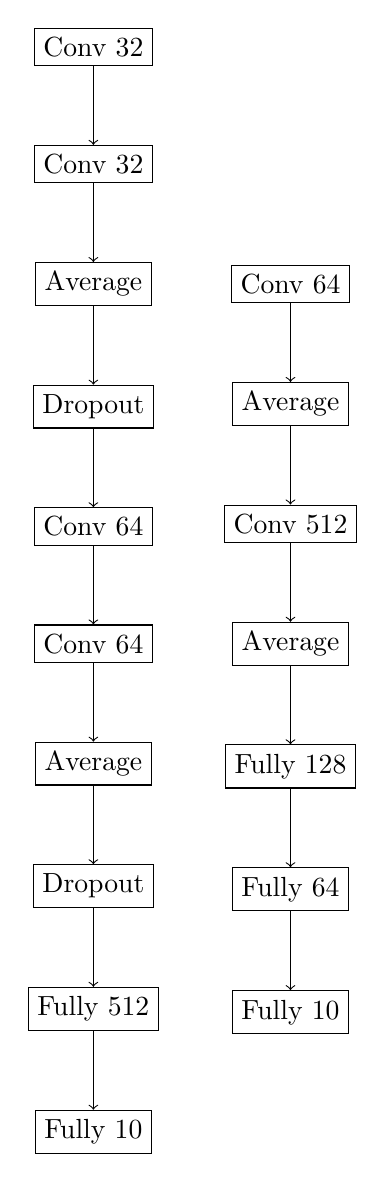
\begin{tikzpicture}
        \tikzstyle{layer}=[rectangle,draw=black]
        \node[layer] (conv_1_1) {Conv 32};
        \node[layer] (conv_1_2) [below=of conv_1_1] {Conv 32};
        \node[layer] (conv_1_3) [below=of conv_1_2] {Average};
        \node[layer] (conv_1_4) [below=of conv_1_3] {Dropout};
        \node[layer] (conv_1_5) [below=of conv_1_4] {Conv 64};
        \node[layer] (conv_1_6) [below=of conv_1_5] {Conv 64};
        \node[layer] (conv_1_7) [below=of conv_1_6] {Average};
        \node[layer] (conv_1_8) [below=of conv_1_7] {Dropout};
        \node[layer] (conv_1_9) [below=of conv_1_8] {Fully 512};
        \node[layer] (conv_1_10) [below=of conv_1_9] {Fully 10};
        \draw[->] (conv_1_1.south) -- (conv_1_2.north);
        \draw[->] (conv_1_2.south) -- (conv_1_3.north);
        \draw[->] (conv_1_3.south) -- (conv_1_4.north);
        \draw[->] (conv_1_4.south) -- (conv_1_5.north);
        \draw[->] (conv_1_5.south) -- (conv_1_6.north);
        \draw[->] (conv_1_6.south) -- (conv_1_7.north);
        \draw[->] (conv_1_7.south) -- (conv_1_8.north);
        \draw[->] (conv_1_8.south) -- (conv_1_9.north);
        \draw[->] (conv_1_9.south) -- (conv_1_10.north);
        \node[layer] (conv_2_1) [right=of conv_1_3] {Conv 64};
        \node[layer] (conv_2_2) [below=of conv_2_1] {Average};
        \node[layer] (conv_2_3) [below=of conv_2_2] {Conv 512};
        \node[layer] (conv_2_4) [below=of conv_2_3] {Average};
        \node[layer] (conv_2_5) [below=of conv_2_4] {Fully 128};
        \node[layer] (conv_2_6) [below=of conv_2_5] {Fully 64};
        \node[layer] (conv_2_7) [below=of conv_2_6] {Fully 10};
        \draw[->] (conv_2_1.south) -- (conv_2_2.north);
        \draw[->] (conv_2_2.south) -- (conv_2_3.north);
        \draw[->] (conv_2_3.south) -- (conv_2_4.north);
        \draw[->] (conv_2_4.south) -- (conv_2_5.north);
        \draw[->] (conv_2_5.south) -- (conv_2_6.north);
        \draw[->] (conv_2_6.south) -- (conv_2_7.north);
    \end{tikzpicture}
    \caption{Long and short CNNs}
    \label{fig:cnns}
\end{figure}

When looking a the loss functions---figures \ref{fig:simple_loss},
\ref{fig:thin_loss}, and \ref{fig:wide_loss}, we see evidence of eventually
overfitting in all the models. 

\begin{figure}
    \centering
    \begin{tikzpicture}
        \begin{axis}[xlabel={Epochs}, ymin=0, ymax=1]
            \addplot table[x=Step,y=Value,col sep=comma]{simple_train_loss.txt};
            \addlegendentry{Training Loss};
            \addplot table[x=Step,y=Value,col sep=comma]{simple_valid_loss.txt};
            \addlegendentry{Testing Loss};
        \end{axis}
    \end{tikzpicture}
    \caption{Simple ANN Loss}
    \label{fig:simple_loss}
\end{figure}

\begin{figure}
    \centering
    \begin{tikzpicture}
        \begin{axis}[xlabel={Epochs}, ymin=0, ymax=1]
            \addplot table[x=Step,y=Value,col sep=comma]{thin_train_loss.txt};
            \addlegendentry{Training Loss};
            \addplot table[x=Step,y=Value,col sep=comma]{thin_valid_loss.txt};
            \addlegendentry{Testing Loss};
        \end{axis}
    \end{tikzpicture}
    \caption{Long, Thin CNN Loss}
    \label{fig:thin_loss}
\end{figure}

\begin{figure}
    \centering
    \begin{tikzpicture}
        \begin{axis}[xlabel={Epochs}, ymin=0, ymax=1]
            % \addplot table[x=Step,y=Value,col sep=comma]{wide_train_loss.txt};
            % \addlegendentry{Training Loss};
            % \addplot table[x=Step,y=Value,col sep=comma]{wide_valid_loss.txt};
            % \addlegendentry{Testing Loss};
        \end{axis}
    \end{tikzpicture}
    \caption{Short, Wide CNN Loss}
    \label{fig:wide_loss}
\end{figure}

\section{Related Work}
\subsection{Capsule Networks}
Capsule networks, as discussed in \cite{sabour2017dynamic}, are neural networks
whose perceptrons output vectors. The vectors carry a probability of a features
existence in the magnitude and information about the feature in question in the
direction. Routing from one layer to the next is determined by agreement of
their outputs, where agreement is measured by the scalar product between two
vectors. With the handwritten MNIST data set, the authors demonstrate that
capsule networks are more resilient to affine transformations than traditional
convolutional networks.

For all but the first layer of capsules, the input to a capsule \(s_{j}\) is the
weighted sum over all prediction vectors \(\hat{u}_{j|i}\), which is formed by
multiplying the previous layer output \(u_{i}\) by a weight matrix \(W_{ij}\).
\begin{align*}
    \hat{u}_{j|i} & = W_{i j} u_{i} \\
    s_{j} & = \sum_{i} c_{i j} \hat{u}_{j|i}
\end{align*}
The final output \(v_{j}\) is normalized so the output is like a probability.
\[v_{j} = \frac{\|s_{j}\|^{2}}{1 + \|s_{j}\|^{2}}\frac{s_{j}}{\|s_{j}\|}\]
The \(c_{ij}\) are the coupling coefficients that are learned through the
dynamic routing process. These coupling coefficients from capsule \(i\) and all
capsules in the subsequent layer sum to 1 and are determined by a routing
softmax whose initial logits \(b_{ij}\) are the log prior probabilities that
capsule \(i\) should be routed to capsule \(j\).
\[c_{ij} = \frac{\exp\left(b_{ij}\right)}{\sum_{k} \exp\left(b_{ik}\right)}\]
The log priors can be learned alone with the other weights. The coupling
coefficients can then be refined by measuring the aggreement between the current
output \(v_{j}\) of each capsule \(j\) in the subsequent layer and the
prediction vector \(u_{j|i}\) made by capsule \(i\) in the current layer.
Agreement is measured by the dot product \(v_{j}\cdot u_{j|i}\).

\subsection{Random Erasing Data Augmentation}
For \cite{zhong2017random}, the data augmentation method of randomly replacing
rectangular regions with noise was used in the CIFAR-10, CIFAR-100, and
Fashion-MNIST data sets. Using this method with various network architectures,
the authors were able consistently to improve on the test error rates across
data sets. The size of the erased region and the regions' aspect ratio was
allowed to vary between a preset minimum and maximum. And the location of the
erased region was allowed to be random, so long as the region fit within the
image size. The authors also experimented with randomly flipping images and
randomly cropping images and found that random erasure was complementary in
these other two data augmentation techniques. They also compared their method
with randomly adding noise to the images and found that these methods failed to
improve the test accuracy. The paper also went into the usefulness of random 
erasure for other visual recognition tasks such as object detection.

\subsection{Branching and Merging Convolutional Networks}
In \cite{byerly2020branching}, the authors achieve great results on
handwriting MNIST by using neural networks that branch. They do this in order to
utilize different levels of abstraction, work with different receptive fields,
and allow information learned early on to be easily accessed at the moment of
classification. The network architecture starts with three convolutional layers,
then branches to either two capsule network layers or to another set of three
convolutional layers the similar branch once more. The results of the three
branches of capsule networks are summed, stacked into a 3-vector for each class,
summed again, and then sent through a softmax layer. Three merging strategies
were tried: one in which the merge weights were equal and not learnable,
a second in which the merge weights were initially equal but learnable, and a
final one in which the merge weights were randomly initialized and learable.
Noteably, the authors cite \cite{hinton2014CNNs} where Geoffrey Hinton argues
against pooling as support for their decision to not use any form of pooling.

Data augmentation was applied to their MNIST dataset where, among other
techniques, the images were randomly rotated by an angle between \(\pm 30\)
degrees, randomly translated up to the point where the bounding box of the digit
sits on the edge of the image, and random 4×4 patch erasure. For all of the
three merging strategies, 32 trails were performed with 300 epochs each. The
strategy where the merge weights were unlearnable achieved a new state of the
art 99.79\% accuracy. The randomly initialized merge weights achieved a max
accuracy of 99.78\%. And the previous state of the art had a max accuracy of
99.77\%. As for ensemble learning, the authors surpassed the previous state of
the art using an ensemble of 4,544 by getting an accuracy of 99.83\% with an
ensemble of 44.

\subsection{Self-Training with Noisy Student}
The paper \cite{xie2019selftraining} is interesting because they used unlabeled
images to improve ImageNet classification. They trained a teacher model on
labeled images, used the teacher to generate pseudo-labels on the unlabeled
images, and trained a noised student model on the labeled and pseudo-labeled
images. This process is iterated by making an old student a new teacher with a
new student. The teacher is not noised when generating pseudo-labels in order to
keep them as accurate as possible. The student is noised with data augmentation
via RandAugment \cite{cubuk2019randaugment} providing input noise and via
dropout and stocastic depth to providing model noise. This makes the student,
which is often a larger model than the teacher, more accurate and more robust
than its teacher. Finally, the authors employ data filtering and class balancing
by filtering images that the teacher model has low confidence in, and duplicate
unlabeled images in classes where there aren't enough images.

The architecture used are EfficientNet \cite{tan2019efficientnet} variants, a
smaller variant for the teacher and a larger variant for the student. This noisy
student approach produced state-of-the-art results on ImageNet. It even beats
out FixRes ResNeXt-101 WSL which employs 3.5B images with tags while using only
300M unlabeled images. Further, Noisy Student gets state-of-the-art robustness
results on ImageNet-A, ImageNet-C, and ImageNet-P.

\subsection{Wide Residual Networks}
The authors of \cite{Zagoruyko_2016} demonstrate that residual networks
\cite{He_2016_CVPR} with decreased depth and increase width, which they call
wide residual networks, are far superior to their thin, deep counterparts. They
experimented with a number of types of residual blocks and found that a sequence
of two \(3\times 3\) convolutional layers do best. Then the paper discusses the
effects of multiplying the number of features in each convolutional layer. It
states that having this multiplier \(k\gt 1\) can generate better results with a
shallower network than when the network is deep and thin, \(k = 1\). They
demonstrate great results for CIFAR-10, CIFAR-100, and SVHN.

\bibliography{bibliography}
\section{Appendix}
\subsection{Source Code}
\lstinputlisting[float=*,linerange=11-25,label=lst:in01,caption={Preamble}]{TensorFlow.py}
\lstinputlisting[float=*,linerange=31-34,label=lst:in02,caption={Reshaping inputs}]{TensorFlow.py}
\lstinputlisting[float=*,linerange=42-46,label=lst:in03,caption={Simple ANN definition}]{TensorFlow.py}
\lstinputlisting[float=*,linerange=52-54,label=lst:in04,caption={Simple ANN compile}]{TensorFlow.py}
\lstinputlisting[float=*,linerange=60-62,label=lst:in05,caption={Simple ANN fit}]{TensorFlow.py}
\lstinputlisting[float=*,linerange=76-94,label=lst:in06,caption={First CNN definition}]{TensorFlow.py}
\lstinputlisting[float=*,linerange=100-101,label=lst:in07,caption={First CNN fit}]{TensorFlow.py}
\lstinputlisting[float=*,linerange=113-117,label=lst:in08,caption={First CNN compile}]{TensorFlow.py}
\lstinputlisting[float=*,linerange=152-170,label=lst:in09,caption={Second CNN definition}]{TensorFlow.py}
\lstinputlisting[float=*,linerange=176-178,label=lst:in10,caption={Second CNN compile}]{TensorFlow.py}
\lstinputlisting[float=*,linerange=184-187,label=lst:in11,caption={Second CNN fit}]{TensorFlow.py}
\end{document}
